\newcommand{\micareviewroot}{../../runs/published/20261021_062155_m2-1600nm-budgeted-r-t-exploration-review_c7387b}
\begin{frame}{A Second Specimen: Mica}
\small
Mica is another specimen studied by Amir for which we want a model (sample M2, 1600 nm).
\par\vspace{0.1cm}
\begin{columns}[c,onlytextwidth]
\begin{column}{.68\textwidth}
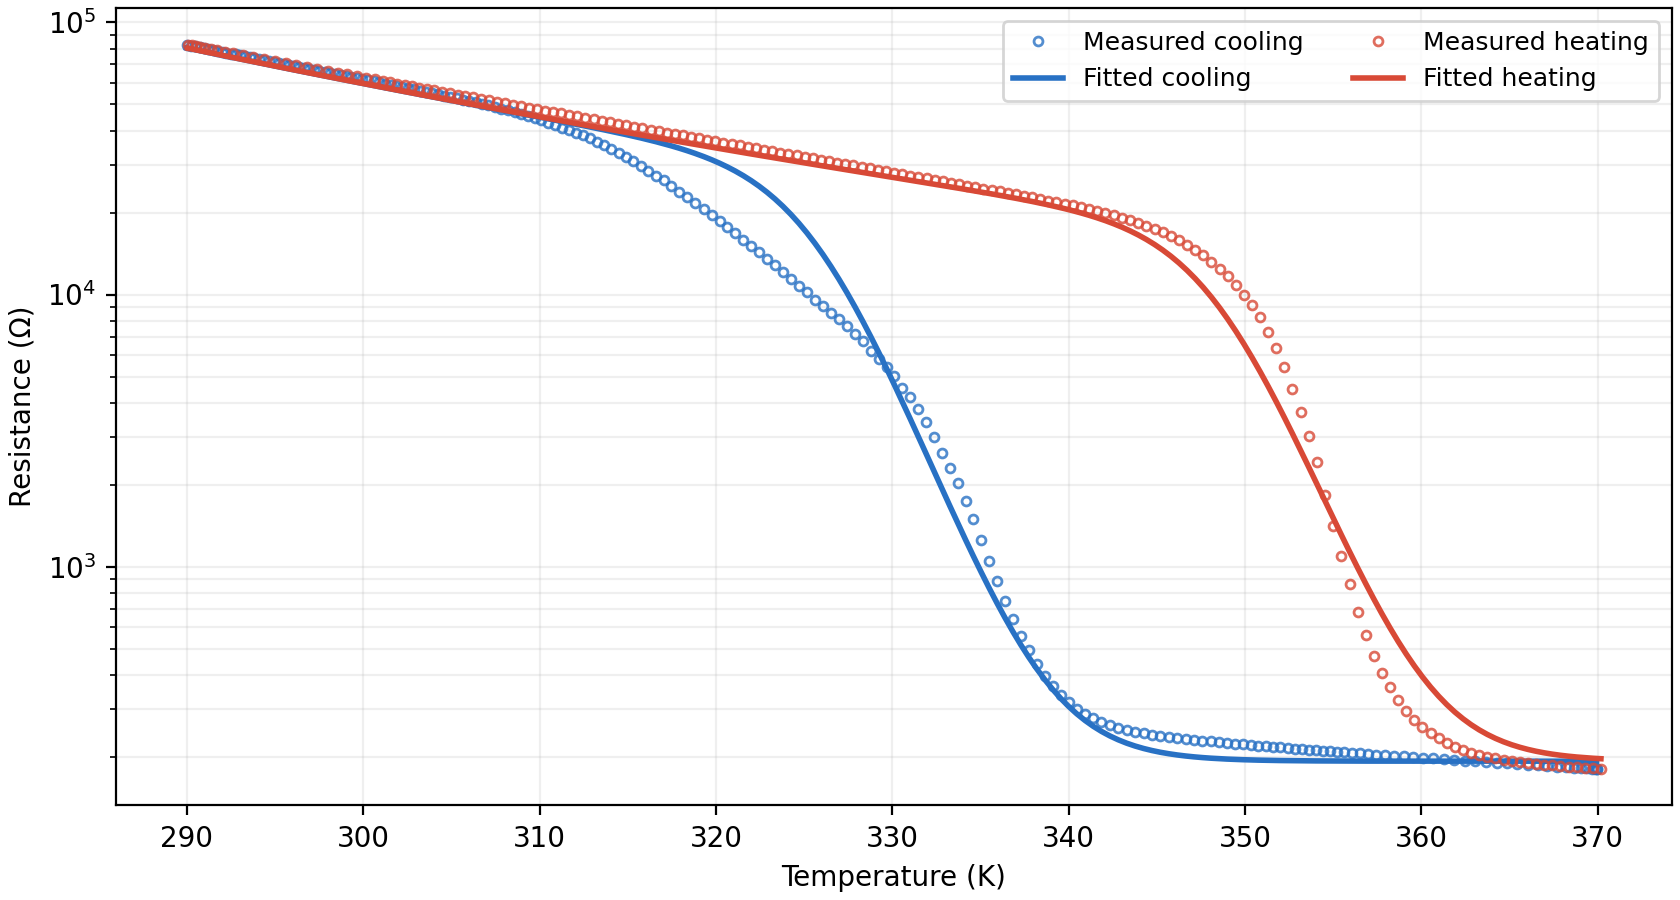
\includegraphics[width=\textwidth]{mica_rt_curve.png}
\end{column}
\begin{column}{.30\textwidth}
\footnotesize
\begin{tabular}{@{}lr@{}}
\toprule
\textbf{Fitted parameter} & \textbf{Mica}\\
\midrule
\(R_0\) (\(\Omega\)) & 9.415\\
\(E_a/k_B\) (K) & 2624.40\\
\(R_m\) (\(\Omega\)) & 193.54\\
\(T_c\) (K) & 337.139\\
\(w\) (K) & 22.815\\
\(\beta\) (K\(^{-1}\)) & 0.18294\\
\bottomrule
\end{tabular}
\par\vspace{0.16cm}
Adopt \(T_0=T_{\mathrm{initial}}=298\) K, matching the parameter explorations.
\end{column}
\end{columns}
\par\vspace{0.1cm}\footnotesize
The static fit is approximate: log\(_{10}\) RMSE \(=0.08065\), with systematic transition errors.
\slidesource{374 measured R(T) points, 289.98--370.18 K; review c7387b. The usual static-fit cutoff is 0.05. No specimen calibration is adopted.}
\end{frame}

\begin{frame}{Mica: Exploring the Parameter Domain}
\small
Using Mica's fitted R(T), vary \(C\), \(C_{th}\) and \(S_e\) to examine their
effects on frequency and peak-to-peak voltage, as for the first specimen.
\par\vspace{0.10cm}\centering
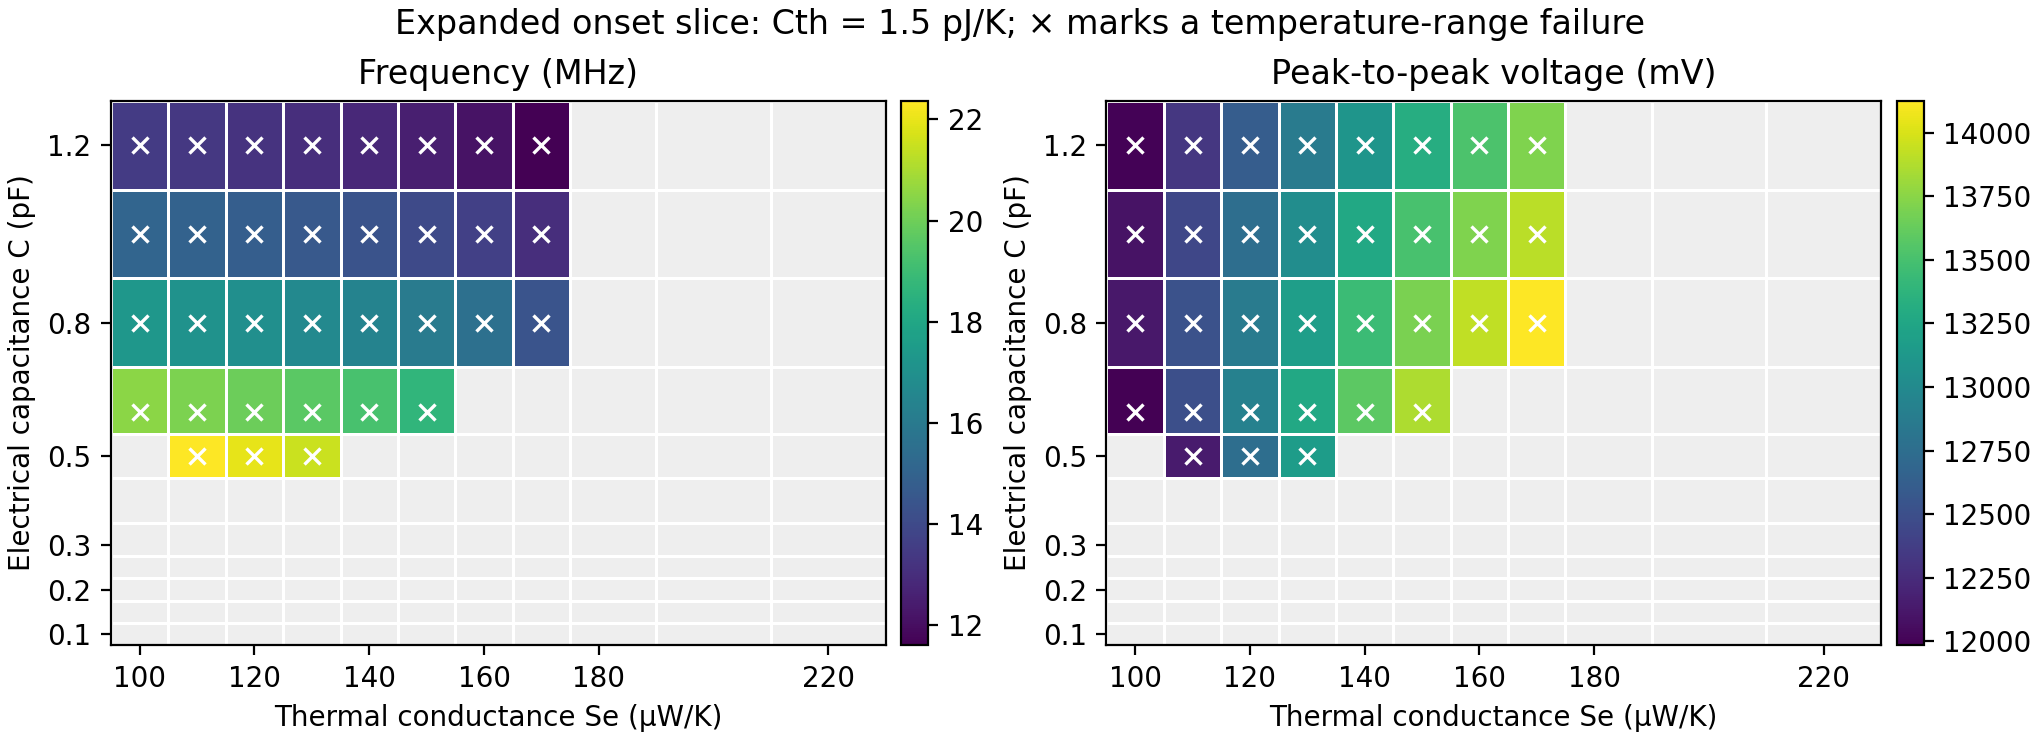
\includegraphics[width=.93\textwidth,height=.48\textheight,keepaspectratio]{mica_parameter_slice.png}
\par\vspace{0.08cm}\raggedright\footnotesize
\textbf{Expanded exploration:} 1,843 additional grid entries; 2,616 in total, including overlaps.
No point passed every check. All detected sustained oscillations still exceeded the measured R(T) temperature range.
\par\vspace{0.14cm}\centering
\localhtmlbutton{mica-map}{Open Mica's latest completed parameter exploration}
\slidesource{Expanded review 226099. Fixed 500 \(\mu\)A, 298 K and assumed \(\gamma=0.95627\). Crosses are excluded diagnostic results; gray cells have no sustained-cycle value. This search does not establish physical boundaries.}
\end{frame}
